\section{Twitter Data and \texttt{twarc2}}\label{sec_dat}
    %Our data consists of **include nb** tweets related to immigration, among Chilean Twitter users before the 2020 elections (from 2020-11-01 to 2022-04-11).
    
    %Collecting the relevant data to analyze is challenging. If from the first step we include bias, the entire analysis risks to be. In the first Twitter query, a search of precise political words  could include bias by oversampling a group. For example, \#FueraDeChile mostly used by the extreme right groups. While searching broad words captures too many irrelevant tweets. For example, in one of our query we ended up scraping tweets from airlines. 
    
    %What we would have liked to do is retrieving tweets related to immigration, then filtering them. However it is not possible since Twitter limits us to 10M tweets and retreiving this amount would be really too much.
        
        
    %    \begin{figure}[!htb]
    %                \centering
    %                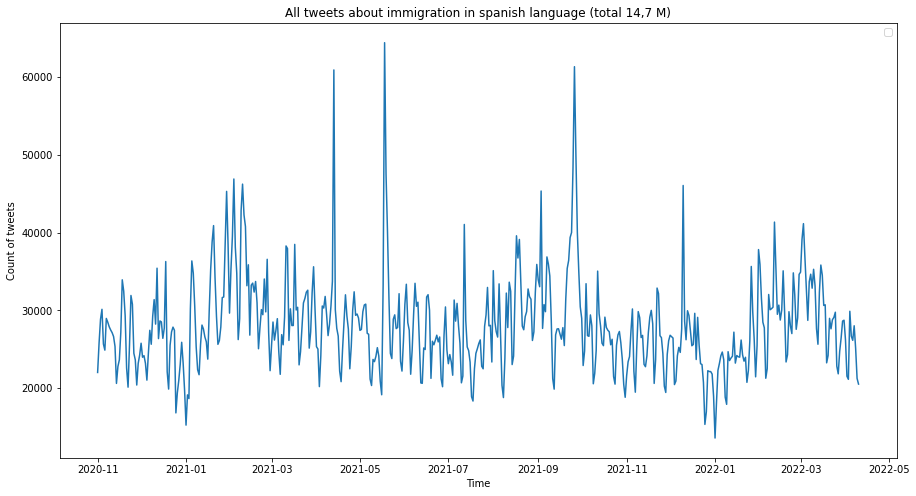
\includegraphics[width=16cm]{figs/14M_tweets}
    %                \caption{Placeholder: Example Figure}
    %                \floatfoot{\it Notes: Some notes
    %                \\ Source: Some data source.}
    %                \label{14M_tweets}
    %            \end{figure}

    Twitter generously provides access for researchers to the full collection of tweets that are currently published on the microblogging website through their {\it Twitter API for Academic Research} service.\footnote{Hence, tweets that get deleted are not available for download.} After being accepted through the company's application procedure, researchers are provided with an allowance of up to 10 M tweets per month to download. To archive Twitter data in \texttt{.json}-file format, we utilize the \texttt{twarc2} Python-based command line tool (see \cite{web_twarc} for more detailed information on the tool). \texttt{twarc2} allows users to specify the corpus of tweets to download by writing queries specifying e.g. specific keywords to filter by, hashtags, retweets, time frames, locations, etc. After downloading, the resulting datafile also includes various metadata for each tweet such as number of likes, retweets, author characteristics, among others (see Appendix \ref{appsec_twarc_meta} for the full list of available metadata). 
        
        \newline\indent
    Unfortunately, the usage of geotagged tweets has declined from 2012 to 2022 following an announcment in mid-2019 that Twitter would remove the option to attach precise geotagging of tweets \citep{kruspe_changes_2021}. This complicates the task of building a country-specific corpus. Solely obtaining geotagged tweets would not yield a sample of sufficient size and raise concerns about the resulting sample being too biased.\footnote{In the case of Chile, there were approximately 50,000 daily geotagged tweets in 2012, which declined to around 20,000 to 30,000 in 2022 as shown in Appendix Figure \ref{appfig_loc_twit_chi_12_22}.} To address this issue we develop a novel methodology to filter non-geotagged tweets to citizens of a given country in Step 3 of Section \ref{sec_meth_gene}.
        
        
        %\newline\indent
    %The aim of this paper is to develop a tool to track political discourse on specific topics in a given country. The tool is designed for political actors to make better informed decisions on where to focus their talking points. Hence, providing an accurate description of the sentiments of the right Twitter users is important. Including tweets by non-citizens (such as registered voters in other countries) would induce noise in the metrics and blur the picture. 

        %\newline\indent
    %In mid-2019, Twitter announced that they would remove the option to attach precise geotagging of tweets \citep{kruspe_changes_2021}. Previous to the policy change, multiple privacy concerns regarding the feature were voiced \citep{drakonakis_please_2019, fiesler_2018_participant, park_2017_protecting}. Unfortunately, this change means that the usage of geolocated tweets has declined from 2012 to 2022. In the case of Chile, there were approximately 50,000 geotagged tweets on a daily basis in the year of 2012, which has declined to around 20,000 to 30,000 in 2022  (see Appendix Figure \ref{appfig_loc_twit_chi_12_22}). Solely obtaining geotagged tweets would therefore not yield a sample of sufficient size and raise concerns about the resulting sample being too biased. We therefore have developed a novel methodology to filter non-geotagged tweets to citizens of a given country. This methodology is presented in Section \ref{sec_meth}.